\subsubsection{Aktivitet og intensitet}\label{subsub:ak_int}
Der er en tydelig sammenhæng mellem puls og kroppens reaktion på den fysiske aktivitet, da den maksimale puls for et individ og intensiteten af den fysiske aktivitet har en lineær sammenhæng. Den maksimale puls kan bestemmes for en person ved at trække personens alder fra 220 \citep{CooperBlair2005}.\newline
Ifølge flere studier hænger procenten af den maksimale puls sammen med henholdsvis antallet af forbrændte kalorier, hvorvidt den aerobe udholdenhed trænes, forbedring af den anaerobe tolerance eller forbedring den kardiovaskulære ydeevne\fxnote{hvilket gør, at man kan sprinte længere / er hurtigere, fordi der kommer mere ilt rundt i kroppen}. I sammenhæng med fysisk aktivitet og udførelse kræver kroppen adenosintrifosfat (ATP). Dette molekyle er energi bærende og nedbrydes konstant for energiudvinding. Anaerobe forhold forekommer, når der ikke er en tilstrækkelig mængde ilt til stede i kroppen, hvorfor denne proces er den første, som indtræder under fysisk aktivitet. ATP kan gendannes anaerobt ved spaltning af kreatinfosfat eller kulhydrater under dannelse af mælkesyre.~\citep{Academic2016c,Martini2012,Engelbreth2010} Under aerobe forhold kan ATP gendannes i store mængder igennem den oxidative fosforylering. Denne proces indtræder og dominerer efter 15-20 minutters fysisk aktivitet. 
\citep{Martini2012,Engelbreth2010} \newline
Pulsen er sigende for aktivitetens intensitetsniveau samt den effekt, som aktiviteten kan påføre personen. Et højere intensitetsniveau resulterer i en højere puls og dermed hårdere fysisk aktivitet. Denne sammenhæng mellem intensitetszoner, maxpuls, varighed samt udbytte inddeles i fem zoner og ses på \tabref{tab:PA_Procentpuls}. \citep{Leyland2007,Heartratejournal2015}
%\begin{figure}[H]
%	\centering
%	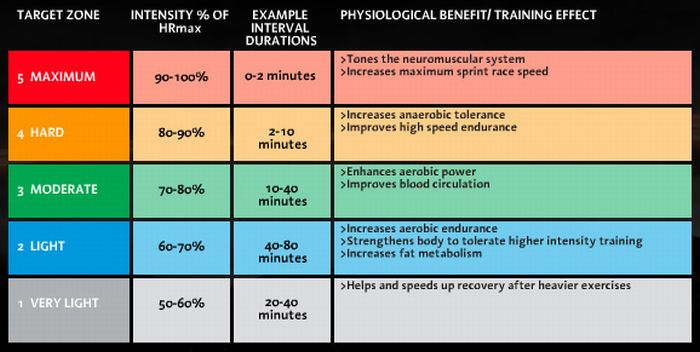
\includegraphics[scale=0.75]{figures/aProblemanalyse/heart-rate-zones.jpg}
%	\caption{På figuren ses fem zoner for kroppens reaktion i forhold til pulsraten. Der ses, at de fem zoner har hver sin påvirkning på kroppen. Det er dog også anbefalet, at varigheden i hver zone bliver lavere desto hårdere aktiviteten er. \citep{Heartratejournal2015}}
%	\label{fig:PA_Procentpuls}
%\end{figure}
\begin{table}[H]
	\centering
	\resizebox{\textwidth}{!}{%
	\begin{tabular}{@{}llll@{}}
		\rowcolor[HTML]{C0C0C0} 
		\multicolumn{1}{c}{\cellcolor[HTML]{C0C0C0}Zoner} & \multicolumn{1}{c}{\cellcolor[HTML]{C0C0C0}\begin{tabular}[c]{@{}c@{}}Procent\\ af maxpuls [\%]\end{tabular}} & \multicolumn{1}{c}{\cellcolor[HTML]{C0C0C0}\begin{tabular}[c]{@{}c@{}}Aktivitetens\\Varighed [min]\end{tabular}} & \multicolumn{1}{c}{\cellcolor[HTML]{C0C0C0}Fysisk udbytte}    \\
		\multicolumn{1}{l}{5 - Maksimum}                & \multicolumn{1}{l}{90-100} & \multicolumn{1}{l}{0-2} & \multicolumn{1}{l}{Træner det neuromuskulære system og øger maksimal sprinthastighed.}   \\ \hline
		\multicolumn{1}{l}{4 - Hård}                    & \multicolumn{1}{l}{80-90}  & \multicolumn{1}{l}{2-10} & \multicolumn{1}{l}{Forbedrer den anaerobe tolerance og øger højhastigheds udholdenhed.}     \\ \hline
		\multicolumn{1}{l}{3 - Moderat}                 & \multicolumn{1}{l}{70-80}  & \multicolumn{1}{l}{10-40} & \multicolumn{1}{l}{Øger aerob power og forbedrer blodcirkulationen.}      \\ \hline
		\multicolumn{1}{l}{2 - Let}                     & \multicolumn{1}{l}{60-70}  & \multicolumn{1}{l}{40-80} & \multicolumn{1}{l}{\begin{tabular}[c]{@{}l@{}}Forbedrer den aerobe udholdenhed, styrker kroppen til høj intens\\ arbejde og øger fedtmetabolismen.\end{tabular}} \\ \hline
		\multicolumn{1}{l}{1 - Meget let}               & \multicolumn{1}{l}{50-60}  & \multicolumn{1}{l}{20-40} & \multicolumn{1}{l}{\begin{tabular}[c]{@{}l@{}}Hjælper og øger hastigheden af genopbygningen af musklerne efter\\ hårdt.\end{tabular}} \\ \hline
	\end{tabular}
	}
	\caption{I tabellen ses fem intensitetszoner, som bestemmes ud fra maxpuls. Der angives en varighed for optimal udbytte inden for hver intensitetszone, som hver har forskelligt fysisk udbytte. (Modificeret) \citep{Heartratejournal2015}}
	\label{tab:PA_Procentpuls}
\end{table} \vspace{-0.5cm}
%Det er dog omdiskuteret, hvorvidt zone 1 og 2 er de fortrukne, hvis ønsket er at tabe sig. Der forbrændes flere kalorier ved højintens aktivitet, altså i zone 4-5. I de lavintense zoner forbrændes kalorier fra fedtceller istedet for glykogen fra muskler, hvorfor kroppen efterfølgende vil lagre kalorier i fedtcellerne, som lider underskud. Hvis man derimod dyrker højintens arbejde, som svarer til zone 4 eller 5, vil glykogenen i musklerne forbrænde, og kalorier sendes derfor til musklerne, så de kan repareres og fortsætte arbejdet. De højintense zoner kan oftest ikke opretholdes over lang tid. \fxnote{Moderat intensitet svarer til 40-59\% af den maksimale iltoptagelse, eller 40-59\% af pulsreserven (maxpuls – hvilepuls), eller 64-74\% af maxpuls eller 12-13 RPE (rate of percieved excertion, Borgskala) og er yderligere defineret som fysisk aktivitet hvor man bliver lettere forpustet men hvor samtale er mulig. \citep{Kiens2007}} \citep{Martini2012,Leyland2007,Heartratejournal2015}. \newline
Pulsen er en sigende faktor for aktivitetens fokus. Dette medfører, at pulsen er bestemmende for intensiteten, varigheden og udbyttet. Intensiteten kan også bestemmes ud fra maksimal iltoptagelse, som er en betegnelse for, hvor meget ilt der optages i minuttet. Derudover kan det bestemmes ud fra Borg skalaen, som er en subjektiv vurdering af hvor hård en given aktivitet er. \citep{Kiens2007}




